% This is part of a Thesis Template by Salvador Rodriguez-Gomez.
% This template is inspired in part by several other templates.
% It is distributed under the Creative Commons Attribution-ShareAlike license.
% http://creativecommons.org/licenses/by-sa/3.0/

%\begin{savequote}[0.49\textwidth]
%Never trust a computer you can't throw\\ out a window.
%\qauthor{Stephen Wozniak}
%\end{savequote}
\chapter{Methodology}
\label{chp:methos}
\epigraph{Never trust a computer you can't throw out a window.}{Stephen Wozniak}
In this chapter, we will discuss the different techniques employed in our study. The main methodology used in this study is Molecular Dynamics (MD) simulation, in which particles trajectories are calculated by integrating the equations of motion. Energy minimisation calculations (EM) are used too. Here, we minimise the total energy of the lattice in order to determine the structure, employing interatomic potentials. In order to perform simulations of adsorption of guest molecules in the pore of the structures, Monte Carlo (MC) simulations were used. Moreover, we have verified some of the structural changes and point-charges calculations with electronic structure techniques using Density Functional Theory (DFT) i.e. quantum calculations. DFT is a powerful but time consuming technique, so we only use it in few key cases, in order to check the results obtained with classical calculations.

\section{Molecular Dynamics}
Intuitively, Molecular Dynamics simulations are the \textit{simplest} type of simulation: particles move around in the system, following trajectories determined by Newton's laws (or by the Hamilton Equations \ref{ecuaciones_canonicas}). In an iterative scheme, the forces they exert on one another are calculated from their positions; based on the forces, the velocities are updated; and these velocities, kept fixed for one time-step $\tau$, yield the new positions one time-step away.

The velocity-Verlet algorithm is the most widely used method for integrating the equations of motion \cite{frenkel1996understanding}. This is implemented in most of simulations codes according to the following equations:
\begin{equation}
\label{verlet1}
\vec{r}_i(t+\tau)=\vec{r}_i(t)+\vec{v}_i(t)\tau +\frac{\vec{f}_i(t)}{2m}\tau^2+\mathcal{O}(\tau^3)
\end{equation}
\begin{equation}
\label{verlet2}
\vec{v}_i(t+\tau)=\vec{v}_i(t)+\frac{\vec{f}_i(t)+f_i(t+\tau)}{2m}\tau+\mathcal{O}(\tau^3)
\end{equation}
where $\vec{r}_i(t)$, $\vec{v}_i(t)$ and $\vec{f}_i(t)$ are the position, velocity and force vector at time $t$, respectively. $\tau$ is the time-step and $m$ the mass of the atom $i$. Note that this algorithm is time-reversible. An unphysical drift in the energy appears after long integration time or as a results of the use of large time-steps, $\tau$. To test this energy drift for a given time-step after $\lambda$ integration steps, we can check the integration validity by requiring the drift is lower than a typical energetic value $\delta$:
\begin{equation}
\label{verlet3}
\sum_{i=1}^{\lambda}{\norm{1-\nicefrac{E(i\tau)}{E(0)}}}< \delta\lambda
\end{equation}

There are several ensembles in which we can run calculations, depending on the conserved quantities: $NVE$, $NVT$, $NPT$, etc. In this thesis, we mainly use the $NVT$ and $NPT$ ensembles. The numerical integration was performed using the Nose-Hoover style non-Hamiltonian equations of motion, which are designed to generate positions and velocities sampled from $NVT$ and $NPT$ ensembles following the scheme of \citet{martynatobiasklein,martyna}.

The ergodic hypothesis states that ensembles averages can be obtained from time averages. So, the time average value, $\langle\ldots\rangle_t$, of a generic property $A$ can be obtained by the following expression
\begin{equation}
\label{eq:expected_value_time_average}
\langle A \rangle_t = \lim_{t\rightarrow\infty}{\frac{1}{t}\int{dt A(x,t)}}.
\end{equation} where $x\equiv\{\vec{r}^N\}$. If Equation \ref{eq:expected_value_ensemble} is equal of the Equation \ref{eq:expected_value_time_average} the system is \textbf{ergodic}.

An important dynamic quantity is the self-diffusivity coefficient $D^\alpha_s$ (in the directions $\alpha=x,y,z$) of $N$ particles, which can be computed by evaluating the mean-square displacement, which reads in three dimensions
\begin{equation}
\label{eq:msd}
D_s^\alpha=\frac{1}{2N}\left\langle \sum_{i=1}^N{\left(r_{i\alpha}(t)-r_{i\alpha}(0)\right)^2}\right\rangle_t
\end{equation} where $r_{i\alpha}$ is the $\alpha$-component of the center-of-mass of particle $i$. The directionally averaged diffusion coefficient is given by
\begin{equation}
\label{eq:diffusion}
D=\frac{D_x+D_y+D_z}{3}
\end{equation}

We have used the order-$n$-algorithm incorporated in the RASPA code \cite{Dubbeldam2009,RASPA_code} to measure accurate mean-square displacements at long times in a fast way.

\section{Lattice energy minimisation}
In the previous Chapter \ref{chap_intro}, in Section \ref{sc:models}, different models for calculating the energy of the systems have been presented. We are interested in finding the minimum state of the system.\footnote{After some considerations can be proved that, under certain conditions, the state of energy minimum state is the most probable.} However, the calculations presented in this section are performed at $T=0 K$. That is, they do not include thermal effects. This state corresponds to a minimum in the potential energy hypersurface, in which:
\begin{equation}
\label{minimum}
\frac{\partial\mathcal{U}(\vec{r}^N)}{\partial r_i}=0\qquad \forall i=1,\ldots,N
\end{equation} where $\mathcal{U}(\vec{r}^N)$ is the total potential energy of the system, as defined in Equation \ref{forcefield}, and $N$ is the number of atoms.

Transition states and local minima also satisfy Equation \ref{minimum}, therefore it is necessary to calculate the second derivative to distinguish between a minimum and a transition state \VIR{(see Figure \ref{fgr:PES})}.
\begin{figure}[ht]
  \centering
  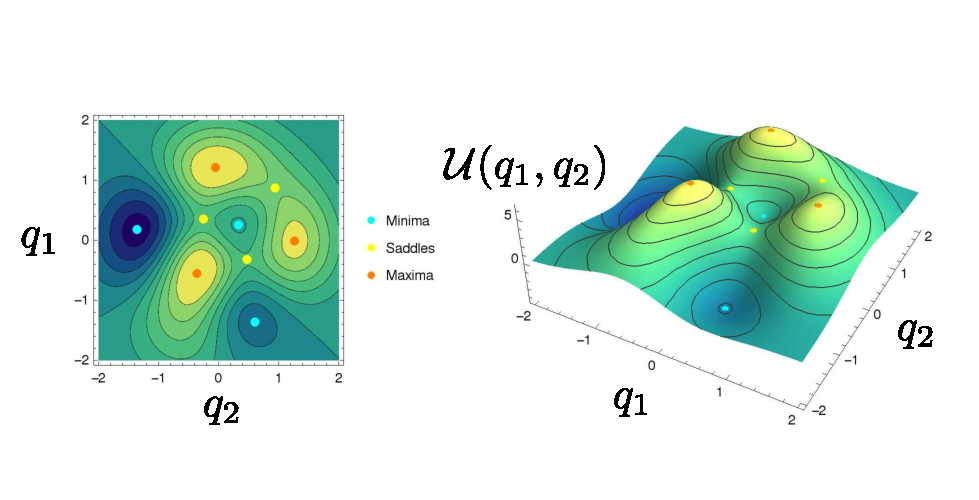
\includegraphics[width=0.9\textwidth]{./methodology/PES.eps}
  \caption{\VIR{Cartoon of the potential energy surface of two generalised coordinates $\mathcal{U}(q_1,q_2)$ in a fictional system.
  Local and global minima (cyan dots) and maxima (red dots) and saddle points (yellow) are indicated on the surface.}
  \label{fgr:PES}
  }
\end{figure}

There are several minimisation algorithms. The simplest algorithm is the \textbf{Steepest Descents} (SD) method \cite{Sheppard2008}, which follows the force vector from an initial configuration to a zero in the force:
\begin{equation}
\label{eq:SD}
\vec{x}_{n+1}=\vec{x_n}-k_n\vec{\nabla}f(\vec{x_n})
\end{equation}
where $k_n$ is a selft-adjustable parameter for each minimisation step. However it is known to converge slowly in \textit{stiff} systems \cite{Press:1996:NRF:232468}. The \textbf{Conjugate Gradient} (GC) method requires both the energy and first derivative evaluations, and is the most efficient method at intermediate distances from the minimum. The CG method improves upon the SD method by following conjugate search directions instead of always following the force. In the LAMMPS code it is implemented the \citet{polak1969note} version of the CG algorithm:
\begin{equation}
\label{eq:CG}
\vec{x}_{n+1}=\vec{x_n}-k_n\vec{h}_n\qquad\text{with}\qquad\vec{h}_n=\vec{\nabla}f(\vec{x}_n)+\gamma_n\vec{h}_{n-1}
\end{equation} where
\begin{equation}
\gamma_n=\frac{\vec{\nabla}f(\vec{x_n})\left( \vec{\nabla}f(\vec{x_n}) - \vec{\nabla}f(\vec{x_{n-1}})\right)^\text{T} }{\norm{\vec{\nabla}f(\vec{x_{n-1}})}^2}
\end{equation} The norm of the gradient is checked to ascertain whether to switch from one method to another. When the system is very close to the energy minimum this method is very slowly convergent. When that happens we switch to the \textbf{Newton-Raphson} method \cite{nocedal2006numerical}, which makes use of the second derivatives of the energy, in order to reach rapidly the energy minimum. Newton-Raphson method approximates the objective function by a quadratic surface at each step and moves to the minimum of that surface:
\begin{align*}
\label{eq:NR}
& f(\vx+\dvx) \simeq f(\vx)+\vec{\nabla}f(\vx)^{\text{T}}\cdot\dvx + \frac{1}{2}\dvx^\text{T}\cdot\mat{H}\cdot\dvx \\
& \vec{\nabla}f(\vx+\dvx) \simeq \vec{\nabla}f(\vx)+ \mat{H}\cdot\dvx \\
& \dvx = -\mat{H}^{-1}\cdot\vec{\nabla}f(\vx)
\end{align*} where $\mat{H}:=(\nicefrac{\partial^2\mathcal{U}}{\partial_{x_i}\partial_{x_j}})$ is the Hessian. This method has a computationally high CPU cost. The most expensive and memory demanding part of Newton-Raphson method is the calculation of the Hessian. The basic Newton-Raphson method requires the Hessian to be non-singular and tends to develop problems if any of its eigenvalues become negative. A simple fix for this is to add a regularisation matrix (often a unit matrix)
\begin{equation}
\dvx = -(\mat{H}+\lambda\mat{S})^{-1}\cdot\vec{\nabla}f(\vx)
\end{equation} \textbf{Rational Function Optimization} (RFO) introduces a step size dependent denominator \cite{Byrd2000}, which prevents the algorithm from taking large steps:
\begin{equation}
f(\vx+\dvx) \simeq f(\vx)+\frac{\vec{\nabla}f(\vx)^{\text{T}}\cdot\dvx + \frac{1}{2}\dvx^\text{T}\cdot\mat{H}\cdot\dvx}{1+\dvx^\text{T}\cdot\mat{S}\cdot\dvx}
\end{equation} 

Both Newton-Raphson and RFO minimisation methods were used to ensure convergence to true energy. However, RFO behaves better than Newton-Raphson in the vicinity of inflection points. Both methods are included in the GULP code \cite{GULP}.
\citet{Baker,Banerjee1985} developed a Eigenvector-Following method. This method solves this limitation of the Newton-Raphson technique by shifting some of the eigenvalues to change their sign and achieve the desired curvature.
This algorithm is incluyed in the RASPA code \cite{Dubbeldam2009b}.

We have used RASPA, GULP and LAMMPS codes \cite{RASPA_code,GULP,lammps_1995} for energy minimisation calculations and to locate saddle points between structural phase-transitions.

